\section{Study Settings}

The main goal of this research work is to replicate Bao et al. study to understand the implications of static analysis algorithms in his results. We also investigate how static analysis can improve the performance of testing tools in the task of identifying malicious behaviors. 

To achieve this general goal, we answer the following research questions. 

\begin{enumerate}[(RQ1)]
\item What is the effective performance of each tool in terms of the number of detected malware ?
\item What benefits of using a hybrid approach, which combines static and dynamic analysis, for mining sandboxes ?
\item What is the impact of static analysis on benchmark results ?
\end{enumerate}

In the first experiment, we executed the benchmark considering 98 pairs of apps for 3 minutes. At this time, we used a new option of the benchmark that disables the static analysis performed by DroidFax. So, we used this experiment to answer the first research questions (RQ1). In the second experiment, we executed all apps with a fake tool called “Joke”, which does not do anything during the benchmark execution, to compute the results without the dynamic analysis influence. With these results, we can answer the last two research question (RQ2 and RQ3).

To assess the effectiveness of mining sandboxes created by each test case generation tools, we run these tools in benign apps and, based on resources sensitives access in this execution, we build their sandbox. Based on this sandbox, we investigate the capacity of detect malicious behaviors in the corresponding malign app. (Figure  \ref{fig:setup}) show all this experimental setup.

\subsection{Settings for RQ1}

\subsection{Settings for RQ2 and RQ3}


\begin{figure*}[h!]
  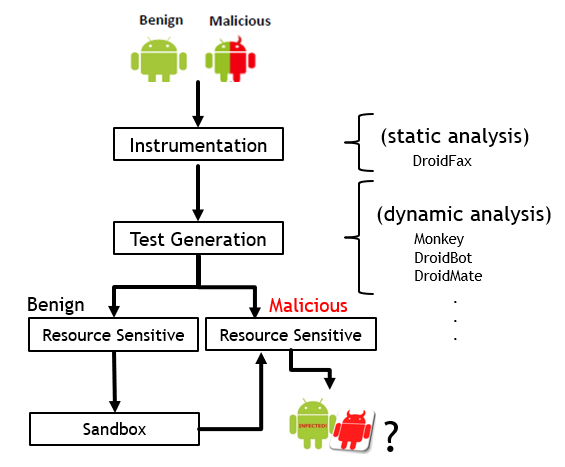
\includegraphics[width=0.5\textwidth]{images/setup.png}
  \label{Experiment setup}
  \caption{Experiment setup}
  \label{fig:setup}
\end{figure*}

\begin{figure*}[ht]
  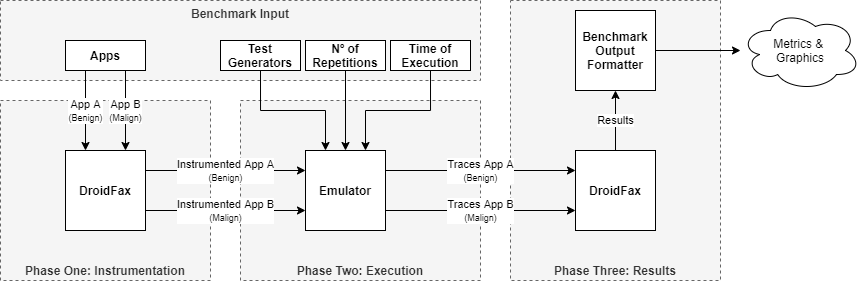
\includegraphics[width=1\textwidth]{images/benchmark3.png}
  \label{benchArq}
  \caption{Benchmark architecture}
  \label{fig:benchArq}
\end{figure*}
